\chapter{Prezentarea sistemelor similare}\label{ch:2sistemeSimilare}

	In momentul de față, acest subdomeniu se află la un nivel mare de răspândire. Există o serie de producători care comercializează sisteme ce permit controlul la distanță al temperaturii, însă au o deficență majoră, și anume, prețul ridicat. Voi prezenta mai multe astfel de sisteme, împreună cu detaliile tehnice ale acestora. 	

\section{Torelectric}
	Termostatul produs de firma Torelectric oferă mai multe modalități de reglare a temperaturii:
	\begin{itemize}
  	\setlength{\itemindent}{2em}
		\itemsep0em
		\item Prin aplicație mobilă
		\item Fizic, utilizând interfața termostatului
		\item Prin comenzi vocale, utilizând Google Home și Alexa
	\end{itemize}
	

	\begin{figure}[H]
    		\centering
    	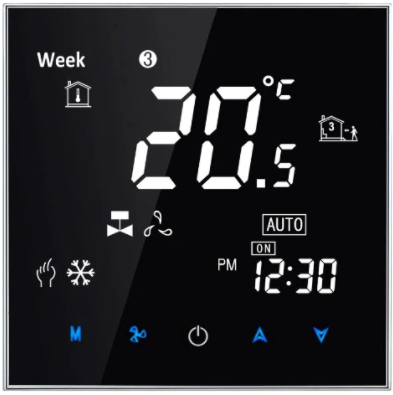
\includegraphics[width=0.3\textwidth]{Torelectric.png}
	\end{figure}

	Ca și caracteristici principale se pot remarca:
	\begin{itemize}
	\setlength{\itemindent}{2em}
		\itemsep0em
		\item Conectivitate: Wi-Fi
		\item Tip alimentare: La retea
		\item Precizie: $\pm 2$ \textdegree{}C sau $\pm 1$ \textdegree{}C
		\item Setare temperatură intre: 5 - 35 \textdegree{}C
		\item Temperatură ambientală: 0 - 45 \textdegree{}C
	\end{itemize}

\section{Honeywell}
\begin{wrapfigure}{l}{0.4\textwidth} 
\centering
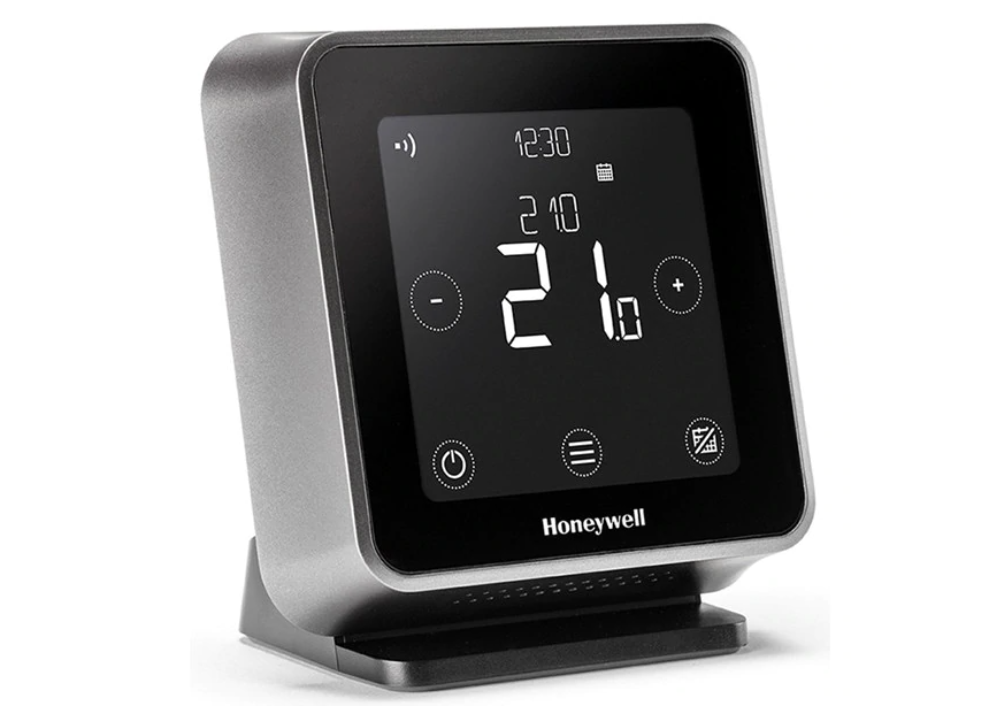
\includegraphics[width=0.4\textwidth]{Honeywell.png}
\end{wrapfigure}
	Termostatul produs de Honeywell se diferențiază față de cel produs de Torelectric prin prezența unor funcționalități inovatoare. Printre particularitățile acestui dispozitiv se remarcă:
	\begin{itemize}
	\setlength{\itemindent}{2em}
		\itemsep0em
		\item Adaptarea temperaturii în funcție de prezența sau absența unor persoane în locuință 
		\item Programarea temperaturilor pentru șapte zile
		\item Controlul de la distanță, oferit de aplicația mobilă
		\item Setarea temperaturii prin comenzi vocale
	\end{itemize}

	Comparativ cu primul sistem prezentat, cel de la Honeywell se deosebește prin tehnologia Geofencing. Acesta știe când imobilul nu este locuit, iar ca urmare, va dezactiva încălzirea. De asemenea, este capabil să detecteze momentul în care locuitorii sunt în apropierea casei, reușind să încălzească până la temperatura setată.
	Un alt avantaj adus de cei de la Honeywell este posibilitatea de a seta temperatura pe decursul a șapte zile, fapt ce asigură un confort sporit, prin adaptarea temperaturii în funcție de diverse intervale orare.

	Caracteristicile tehnice ale acestuia sunt:
	\begin{itemize}
	\setlength{\itemindent}{2em}
		\itemsep0em
		\item Destinat: centrale termice
		\item Suprafata de montare: masă
		\item Tip alimentare: la rețea
		\item Conectivitate: Wi-Fi
	\end{itemize}

	În continuare, voi prezenta două sisteme care reprezintă apogeul evoluției în acest domeniu. Acestea sunt produse de firme cunoscute precum: Google si Ecobee.

\section{Nest}
	Este un termostat inteligent produs de cei de la Google. Acesta oferă funcționalități avansate pentru un management, cât mai eficient, al temperaturii din imobil. 

	Spre deosebire de sistemele prezentate anterior, termostatele produse de Google Nest integrează tehnologii revoluționare pentru a obține un randament cat mai mare.

\vspace{2em}

	Principalele particularități ale acestuia sunt:
	\begin{itemize}
	\setlength{\itemindent}{2em}
		\itemsep0em
		\item Capacitatea de a se programa automat, în funcție de rutina locuitorilor
		\item Menține temperatura setată doar dacă există persoane în imobil, altfel trece automat la o temperatură ce asigură un consum cât mai mic de energie
		\item Control de la distanță de pe laptop, tabletă și telefon
		\item Salvarea unui istoric al consumului de energie
		\item Tehnologie Geofencing
		\item Se pot adăuga senzori pentru mai multe zone
	\end{itemize}

\vspace{2em}

\begin{wrapfigure}[5]{l}{0.4\textwidth}
\centering
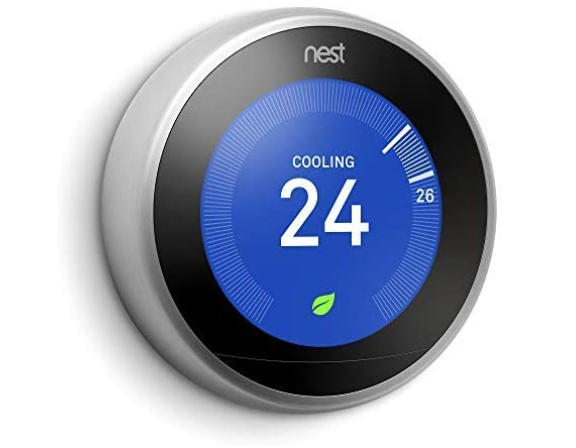
\includegraphics[width=0.4\textwidth]{Nest.png}
\end{wrapfigure}

	Date tehnice:
	\begin{itemize}
	\setlength{\itemindent}{2em}
		\itemsep0em
		\item Sursă de energie: baterii
		\item Tensiune de funcționare: 24 volți
		\item Afișaj digital
		\item Conectivitate: WiFi
	\end{itemize}

\vspace{2em}

\section{Ecobee}
	 Termostatul produs de firma Ecobee concurează cu Google Nest. Acesta oferă, pe lângă funcțiile complexe, posibilitatea de monitorizare detaliată a consumului de energie.
	
\vspace{2em}

	Particularități:
	\begin{itemize}
	\setlength{\itemindent}{2em}
		\itemsep0em
		\item Poate fi controlat prin intermediul unor aplicații precum: Apple HomeKit, Alexa built-in, Google Assistant și SmartThings. De asemenea, oferă posibilitatea de a seta temperatura de pe Android, dar si de pe iOS.
		\item Implementează un algoritm ce permite controlul temperaturii în diverse locuri din imobil. Se pot conecta mai mulți senzori de temperatura la termostat, iar in funcție de informatiile primite de la aceștia, menține o temperatură constantă în locuință.
		\item Ecranul se aprinde atunci când detectează o persoană în apropiere, iar pe lângă informațiile legate de temperatură si umiditate, se afișează si vremea pe decursul a cinci zile.
		\item Este prezentă tehnologia Geofencing
	\end{itemize}

\vspace{2em}

\begin{wrapfigure}[5]{r}{0.4\textwidth}
\centering
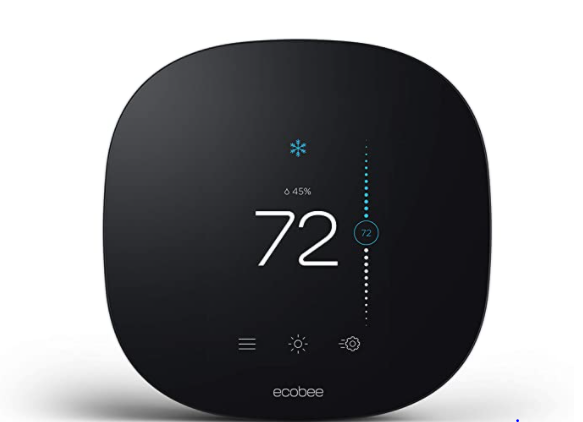
\includegraphics[width=0.4\textwidth]{Ecobee.png}
\end{wrapfigure}
	Date tehnice:
	\begin{itemize}
	\setlength{\itemindent}{2em}
		\itemsep0em
		\item Sursă de energie: baterii sau rețea
		\item Tensiune de funcționare: 24 volți
		\item Ecran tactil
		\item Conectivitate: WiFi
	\end{itemize}
\vspace{2em}

\section{Abordare comparativă a sistemelor prezentate}
	Dacă primele două sisteme prezentate reprezentau soluții mai ieftine, ultimele două sunt recunoscute ca fiind cele mai evoluate termostate existente pe piață. Diferențele esențiale sunt vizibile la nivelul funcționalitaților oferite, dar și al calității.

	Lipsa posibilității de a programa în avans temperaturi pe mai multe intervale orare și zile, de a monitoriza temperatura în mai multe camere, de a stoca un istoric al consumului de energie și de a adapta temperaturile in funcție de rutina locuitorilor, sunt câteva din minusurile termostatelor Torelectric și Honeywell. Google Nest și Ecobee, pe lângă faptul că rezolvă aceste probleme, oferă și o experiență mult mai bună a utilizatorului. Interfețele sunt proiectate în așa fel încât să permită o navigare facilă prin meniurile sistemelor.  

	În continuare, cu ajutorul datelor preluate din [citeaza articolul lui Eric Blank], voi prezenta o analiză comparativă a sistemelor oferite de Google Nest și Ecobee. 

	Termostatul Nest inregistrează fiecare modificare de temperatură pe care utilizatorul o face. După o perioadă de timp, acesta va programa automat temperaturile din imobil în funcție de istoricul de temperaturi setate de utilizator. Ecobee nu prezintă această funcționalitate, dar oferă posibilitatea de a seta temperaturi diferite pe intervale orare diferite. 

	In ceea ce privește controlul prin comenzi vocale, Nest este compatibil cu un număr mai mic de asistenți virtuali(Google Assistant si Alexa). Ecobee este compatibil și cu Siri, fapt ce reprezintă un avantaj, datorită numărului mai mare de potențiali clienți. 

	Tehnologia Geofencing constă în detecția momentului în care imobilul este gol și setarea unei temperaturi ce asigură un consum minim de energie. Totodată, poate detecta dacă locuitorii se apropie de imobil, pentru a ieși din modul economic și a asigura temperatura setată. Geofencing este prezent la ambele termostate, însă la Nest este mai avansat. Poate detecta mai multe telefoane, iar în cazul în care sunt persoane care rămân în locuință și nu au telefonul conectat la Geofencing, prezența acestora este sesizată prin detectoarele de fum Nest, iar modul eco nu va fi activat. Ecobee poate conecta un singur telefon la Geofencing, ceea ce poate reprezenta un dezavantaj.

	  Monitorizarea consumului de energie se face automat, dar cei de la Ecobee au pus mai mult accent pe această parte, iar raportul pe care termostatul îl face este mult mai detaliat. Se analizează datele în decursul a 18 luni și conține informații legate de: consumul total, influența vremii asupra consumului de energie și compară eficiența imobilului cu celelalte din zonă. Pe de altă parte, Nest poate înregistra doar cosumul în decursul a 10 zile. Acesta trimite mail-uri în fiecare lună cu un raport ce conține detalii de consum de energie și face comparație cu luna anterioară.

	Monitorizarea temperaturii se face în mai multe zone din imobil prin intermediul unor senzori adiționali. Cele două termostate incearcă să mențină o temperatură medie în locuință. Senzorii oferiți de Ecobee detectează și dacă se află cineva în încăperea respectivă. 

\section{Comparație cu sistemul prezentat în această lucrare}

	În urma analizei sistemelor existente pe piață, se pot observa două dezavantaje majore. În primul rând, menținerea unor temperaturi exacte în fiecare cameră din imobil este destul de greu de obținut. Chiar dacă se pot adăuga mai mulți senzori de temperatură, termostatele prezentate vor reuși să asigure o temperatură medie la nivel de imobil, și nu o temperatură specifică la nivel de cameră. De asemenea, prețurile acestora sunt destul de ridicate. Prin proiectul de diplomă, am încercat să soluționez aceste probleme. Costurile pieselor pe care le-am utilizat sunt abordabile, iar electrovalvele montate pe returul caloriferelor au rolul de a asigură menținerea temperaturii setate în fiecare cameră.
